\subsection{Präprozesssor für Ruby}

\begin{frame}
\begin{center}
	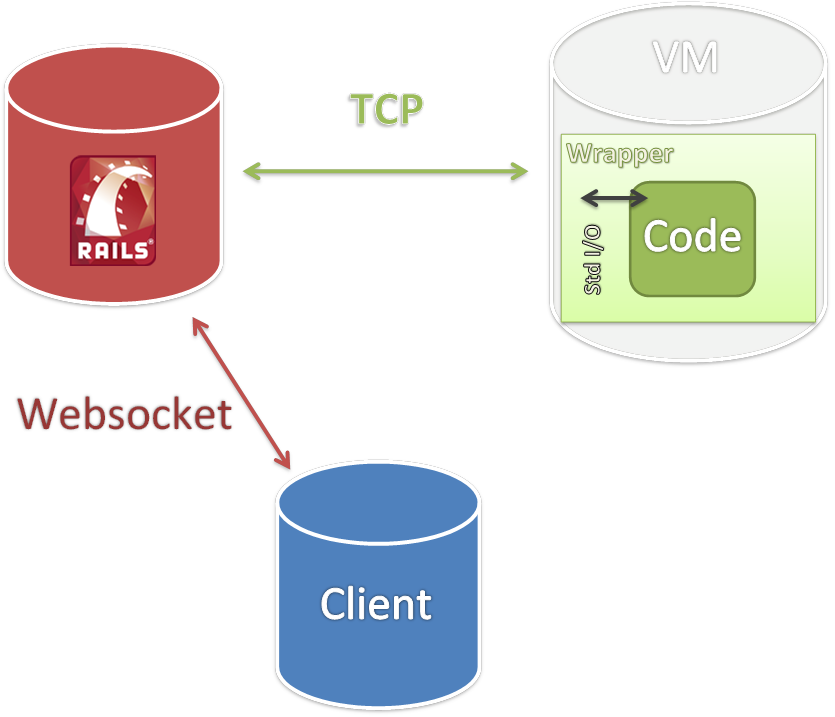
\includegraphics[scale=0.35]{overview}
\end{center}
\end{frame}

\begin{frame}
\frametitle{Idee}
%Ruby, rub, rub! :3
\begin{center}
\includegraphics[scale=0.5]{preprocessor/pics/Idee}
\end{center}
%Spiellogik vor den User code kopieren und den Code für das line highlighting und das Verfolgen von Variablen mit dem nötigen Input füttern.
\end{frame}

\begin{frame}
\frametitle{Erkennung von Sonderfällen}
	\includegraphics[scale=0.70]{preprocessor/pics/CodeArten}
\end{frame}

\begin{frame}
\frametitle{Standard Verfahren}
\inputminted[linenos, numbersep=3pt, tabsize=2, frame=lines]{ruby}{preprocessor/sampleStandard.rb}
\end{frame}

\begin{frame}
\frametitle{Standard Verfahren mit Variablenverfolgung}
  \inputminted[linenos, numbersep=5pt, tabsize=4, frame=lines]{ruby}{preprocessor/sampleDebug.rb}
\end{frame}

\begin{frame}
\frametitle{Verarbeitung mehrzeiliger Strings}
  \includegraphics[scale=1]{preprocessor/pics/MultilineVerarbeitung}
\end{frame}

%\begin{frame}
%\frametitle{Verarbeitung von Case Blöcken}
%\begin{center}
%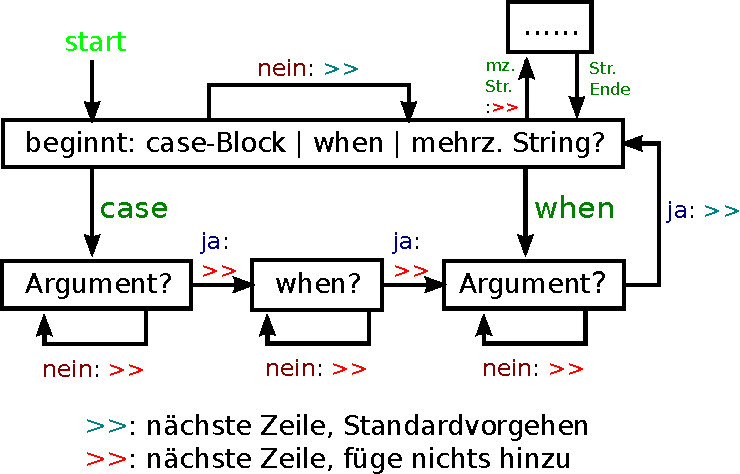
\includegraphics[scale=0.8]{preprocessor/pics/CaseBlockVerarbeitung}
%\end{center}
%\end{frame}

\begin{frame}
%\frametitle{Code: vorher und nachher}
  \begin{columns}
    \column[t]{0.50\textwidth}
\inputminted[linenos, frame=lines, tabsize=2, fontsize=\footnotesize , label=case when einzeilig]{ruby}{preprocessor/CaseB.rb}
    \column[t]{0.50\textwidth}
    \inputminted[linenos, frame=lines, tabsize=2, fontsize=\footnotesize , label=case mehrzeilig]{ruby}{preprocessor/CaseA.rb}
  \end{columns} 
\end{frame}

\begin{frame}
%\frametitle{Code: vorher und nachher}
  \begin{columns}
    \column[t]{.50\textwidth}
\inputminted[ tabsize=2, fontsize=\footnotesize , label=vorher]{ruby}{preprocessor/sampleA.rb}
    \column[t]{.50\textwidth}
    \inputminted[ tabsize=2, fontsize=\footnotesize , label=danach]{ruby}{preprocessor/sampleB.rb}
  \end{columns} 
\end{frame}

\begin{frame}
\frametitle{Beschränkungen für den Nutzer}
  \begin{columns}
    \column[c]{.65\textwidth}
    \begin{itemize}
    \item \textit{return} bei eigenen Funktionen
    \item keine mehrzeiligen Strings der Form             
    \%q[Text des Strings] oder 
    
    \%Q[anderer Text]
    \end{itemize}
    \column[c]{.35\textwidth}
  
\includegraphics[scale=0.15]{preprocessor/pics/Verbotsschild}
  \end{columns} 
\end{frame}